Corresponds to this reference \cite{2014Hassler}. To be honest, I use it as a guideline, but all this can be considered as my own writting.\\

\subsection{Introduction}

Let's say we have a piece of cloth, very elastic, and additionally it is impossible to make holes on it or rip it apart. We can stretch it in one direction, in the other, maybe in both. Twist it, bend it, any contortion or elongation; the only forbidden deformations are any kind of ripping on the cloth. There are ways to analyze all the physical phenomena playing a role while we deform the cloth, but at the end of the day we can with all certainty keep saying that what we have in our hands is (and throughout the process was) still an elastic piece of cloth. This leads us to think there are some properties that were not changed in the process: the color, the texture, the pattern, and so on. That is to say, we know that some properties were unchanged under all the deformations, we can use our senses to perform an analysis. For mathematical objects, since they are abstract, we don't have the advantage of directly using our senses, therefore we need a tool, topology is the one in charge of analyzing the properties that remain unchanged as we stretch or bend such bodies.\\

Topology became a major branch of mathematics during the 20th century, but some of its ideas go back as early as 1736 with the seven bridges of Könisberg problem \cite{konigs}. But for a long time, there was not an obvious way to make use of it in physics or chemistry, and as a consequence it was for a long time used exclusively by mathematicians. In the last decade it has been found that topology is a very useful tool to gain insight into the physics of materials \cite{natTop}. In this section it will be shown how can we use topology to build a system whose applications can potentially lead to an implementation of quantum computing that is very resistant to certain kind of errors.

\subsection{Second quantization and Majorana fermions}

So far we have being treating the operator $c_j$ as an object which destroys a particle located in site $j$, but we can also think of it as the creator of an antiparticle. For example it can create an positron, antiproton, antineutron, etc. When such antiparticles come into contact with their counterparts, namely electron, proton, neutron ..., both annihilate each other. Each particle has it's own antiparticle, this is a direct result of Dirac's equation. Each superhero has it's own villain, but can a superhero be also the villain? Next section will dive further into this idea.

\colorbox{orange}{30.04.19 Rethink the last paragraph, the idea is there, but it might not be well expressed.}

\subsubsection{Majorana fermions}

It was not long since Schrödinger developed his celebrated wave equation that people realized it was not relativistic, i.e. it was not Lorentz invariant. This set the next step for the theoretical community, find a relativistic Schrödinger equation. In 1926 Oskar Klein and Walter Gordon propose a Lorentz invariant version of it, however, it has two important flaws, it could not be used for spin half particles, and as a byproduct had a solution with negative energy\cite{antimatter}. Dirac went on looking for a equation that could be used with fermions (spin half particles), eventually he arrived to the equation discussed in section \ref{dirEq}. This one, nevertheless, kept one of the Klein-Gordon equation flaws, namely, the negative energy solution. Dirac was less shy on this affair, instead of labeling this solution as unphysical, he said this showed that each particle has a mirror antiparticle with almost similar properties, except for the electrical charge. This would not be the only surprise we were going to get from Dirac's equation as we will see soon.\\


Ettore Majorana found another big surprise hidden within Dirac's equation while forcing it to have purely real solutions. For this case he found that the resulting wave functions characterized particles that were at the same time their own antiparticles. As a tribute to him, they were baptized as Majorana fermions or Majorana particles. So in a sense, creating a Majorana particle would be equivalent to creating its antiparticle. Mathematically, we can represent this property through operators as $\gamma_i = \gamma_i^\dagger$. As their fermionic counterparts they also have anticommutation relations, in this case they are 
\begin{equation}
    \{\gamma_k,\gamma_j\} = 2\delta_{kj},
    \label{anticomm}
\end{equation}
where the factor of 2 is there just for convenience as we will see later.\\

Since Majorana's prediction in 1937 there has been and intense search for these fermions in the wild. But so far, nothing conclusive has been obtained. This then lead us to a trivial and a not so trivial question. The former would be: if they are so elusive, why do we care about them? The fact that they have proved to be hard to find might dissuade us from trying to find applications for them. The second question is slightly related to the former, if this fermions cannot be found as elementary particles, is there a way to create them? We can for example look for them as excitations in materials, as with phonons, magnons, plasmons, etc. This approach has advantages, for example it can provide us with ways to create, destroy, and control these particles. From this point on, we will use the term Majorana modes when we refer to Majorana fermions arising from excitations.\\

At this point the reader might suspect that the author has a secret fascination for Majorana modes and wants to see them at any cost. Truth be told, suspicions are almost correct (the fascination is not secret though), however, it is out task to clarify why they can be of importance, and with a little bit of luck encourage the reader to travel this path too. The remaining part of this subsection will be dedicated to lay down the mathematical foundations needed to understand and manipulate these objects.\\

For the fermionic creation and annihilation operators we were able to go from their definition to the anticommutation relations they comply with. But know we find ourselves in a different position, namely we know the commutation relations and a simple property about the operators. We can give this a thought, could we construct the Majorana fermions creation and annihilation operators solely with this properties? We don't have to start from zero, we already know some things, for example the fermionic operators $c_i$ and $c_i^\dagger$, maybe they can help us. Let's write an arbitrary linear combination of both

\begin{equation*}
    \begin{aligned}
        &\gamma_k &= |a|e^{i\phi}c_k + |b|e^{i\omega}c_k^\dagger,
    \end{aligned}
\end{equation*}
given this, the hermitian conjugate operator would be 
\begin{equation*}
    \begin{aligned}
        \Rightarrow\quad & \gamma_k^\dagger &= (|a|e^{i\phi}c_k + |b|e^{i\omega}c_k^\dagger)^\dagger,\\
        && = |a|e^{-i\phi}c_k^\dagger + |b|e^{-i\omega}c_k.
    \end{aligned}
\end{equation*}
\begin{wrapfigure}{l}{0.5\textwidth} % Inline image example
   \begin{center}
     \resizebox {0.35\columnwidth} {!} {
    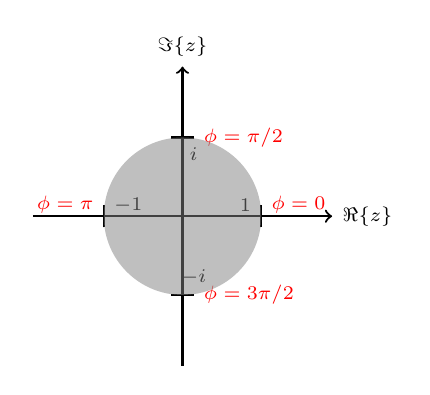
\begin{tikzpicture}
    \begin{scope}[thick,font=\scriptsize]
    %xscale=2
    % Axes:
    % Are simply drawn using line with the `->` option to make them arrows:
    % The main labels of the axes can be places using `node`s:
    \draw [->] (-1.9,0) -- (1.9,0) node [right]  {$\Re\{z\}$};
    \draw [->] (0,-1.9) -- (0,1.9) node [above] {$\Im\{z\}$};

    % Axes labels:
    % Are drawn using small lines and labeled with `node`s. The placement can be set using options
    \iffalse% Single
    % If you only want a single label per axis side:
    \draw (1,-3pt) -- (1,3pt)   node [above] {$1$};
    \draw (-1,-3pt) -- (-1,3pt) node [above] {$-1$};
    \draw (-3pt,1) -- (3pt,1)   node [right] {$i$};
    \draw (-3pt,-1) -- (3pt,-1) node [right] {$-i$};
    \else% Multiple
    % If you want labels at every unit step:
    \draw (1,-4pt) -- (1,4pt)   node [right] {\textcolor{red}{$\phi = 0$}};
    \draw (-4pt,1) -- (4pt,1)   node [right] {\textcolor{red}{$\phi = \pi/2$}};
    \draw (-4pt,-1) -- (4pt,-1)   node [right] {\textcolor{red}{$\phi = 3\pi/2$}};
    \draw (-1,-4pt) -- (-1,4pt)   node [left] {\textcolor{red}{$\phi = \pi$}};

    \draw (1,-4pt) -- (1,4pt)   node [left] {$1$};
    \draw (-4pt,1) -- (4pt,1)   node [below] {$i$};
    \draw (-4pt,-1) -- (4pt,-1)   node [above] {$-i$};
    \draw (-1,-4pt) -- (-1,4pt)   node [right] {$-1$};

    \fi
    \end{scope}
    % The circle is drawn with `(x,y) circle (radius)`
    % You can draw the outer border and fill the inner area differently.
    % Here I use gray, semitransparent filling to not cover the axes below the circle
    \path [draw=none,fill=gray,semitransparent] (0,0) circle (1);
\end{tikzpicture}
}
   \end{center}
   \caption{Unitary circle in the complex plane. In red, the corresponding angles of the polar representation $e^{i\phi}$.}
   \label{unitCircle}
 \end{wrapfigure}
We mentioned earlier that the condition of a Majorana fermion being its own antiparticle would translate mathematically to the equation $\gamma_i = \gamma_i^\dagger$. This leads us to 
\begin{equation*}
    \begin{aligned}
     |a|e^{i\phi}c_k + |b|e^{i\omega}c_k^\dagger &= |a|e^{-i\phi}c_k^\dagger + |b|e^{-i\omega}c_k,\\
     \Rightarrow \quad|a|e^{i\phi} &= |b|e^{-i\omega},\\
     \Rightarrow \quad|b|e^{i\omega} &= |a|e^{-i\phi}.
    \end{aligned}
\end{equation*}
From last two equalities we can conclude two things: $|a| = |b|$ and $\phi = -\omega$. As a consequence our assumptions for the $\gamma_k$ operators get modified to 
$$\gamma_k = |a|e^{i\phi}c_k + |a|e^{-i\phi}c_k^\dagger = |a|(e^{i\phi}c_k + e^{-i\phi}c_k^\dagger).$$
Hence the property $\gamma_i = \gamma_i^\dagger$ is properly covered. Now is time to take care of the anticommutation relations in eq. \ref{anticomm}, so let's calculate\\

 \begin{equation}
    \begin{aligned}[b]
     \{\gamma_k,\gamma_l\} &= \{ |a|(e^{i\phi_k}c_k +  e^{-i\phi_k}c_k^\dagger), |a|(e^{i\phi_l}c_l +  e^{-i\phi_l}c_l^\dagger)\}, \\
     &= |a|^2(\{ e^{i\phi_k}c_k, e^{i\phi_l}c_l\} +  \{ e^{i\phi_k}c_k , e^{-i\phi_l}c_l^\dagger\} +  \{e^{-i\phi_k}c_k^\dagger, e^{i\phi_l}c_l\} +  \{e^{-i\phi_k}c_k^\dagger, e^{-i\phi_l}c_l^\dagger\}),\\
     &= |a|^2(e^{i(\phi_k+\phi_l)}\cancelto{0}{\{ c_k,c_l\}} +  e^{i(\phi-\phi_l)}\{ c_k ,c_l^\dagger\} +  e^{i(-\phi_k+\phi_l)}\{c_k^\dagger, c_l\} +  e^{i(-\phi_k-\phi_l)}\cancelto{0}{\{c_k^\dagger,c_l^\dagger\}}),\\
     &= |a|^2(e^{i(\phi_k-\phi_l)}\cancelto{\delta_{kl}}{\{ c_k ,c_l^\dagger\}} +  e^{i(-\phi_k+\phi_l)}\cancelto{\delta_{kl}}{\{c_k^\dagger, c_l\}}),\\
     &= |a|^2(e^{i(\phi_k-\phi_l)}\delta_{kl} +  e^{i(-\phi_k+\phi_l)}\delta_{kl}).
    \end{aligned}
    \label{34}
\end{equation}
Given last equation, if we set $k=l$ we get that $\{\gamma_k,\gamma_k\} = |a|(e^{i(\phi_k-\phi_k)}\delta_{kk} +  e^{i(-\phi_k+\phi_k)}\delta_{kk}) = 2|a| $. For $k \neq l$ we have $\{\gamma_k,\gamma_l\} = 0$, since $\delta_{kl} = 0$ for this case. This means that we can write our result in a simpler way, that is to say eq. \ref{34} is equivalent to 
\begin{equation*}
    \{\gamma_k,\gamma_l\} = e^{i(\phi_k-\phi_l)}\delta_{kl} +  e^{i(-\phi_k+\phi_l)}\delta_{kl} = 2|a| \delta_{kl}
\end{equation*}
Since these operators have to satisfy the anticommutation relations in eq. \ref{anticomm} this imposes $|a|=1$, then $\gamma_k$ mutates to 
 \begin{equation*}
    \gamma_k = e^{i\phi}c_k + e^{-i\phi}c_k^\dagger.
\end{equation*}
To give a quick rundown. Any operator of this form meets the requirements to be a Majorana operator, i.e. the anticommutator and being its own hermitian conjugate. If we look carefully at this last equation we might realize that we face an overchoice. We are left with the freedom to select any value for $\phi$. This is not a problem per se, nevertheless we have to consider if some options are better than others, and for this it can be beneficial to explore a couple of special cases. If we look at fig. \ref{unitCircle} we can see that there are some special instances for this phase factor, $\phi = 0,\pi$, and $\phi = \pi/2, 3\pi/2$. $\phi = 0, \pi$ results in
\begin{equation*}
    \gamma_k = e^{i0}c_k + e^{-i0}c_k^\dagger = c_k + c_k^\dagger, \qquad \gamma_k = e^{i\pi}c_k + e^{-i\pi}c_k^\dagger = -(c_k + c_k^\dagger),
\end{equation*}
these are the only two combinations that give purely real operators. In fact, it can be considered as just one instance, since the only difference between the two of them is a global phase (in this case $e^{i\pi}$). Furthermore, we have the option $\phi = \pi/2, 3\pi/2$, this one leads to
\begin{equation*}
    \gamma_k = e^{i\pi/2}c_k + e^{-i\pi/2}c_k^\dagger = ic_k -i c_k^\dagger = i(c_k - c_k^\dagger), \qquad \gamma_k = e^{i3\pi/2}c_k + e^{-i3\pi/2}c_k^\dagger = -i(c_k -c_k^\dagger),
\end{equation*}
this time, we get purely imaginary operators. And as in the previous case the only difference between this pair is a global $e^{i\pi}$ phase.\\

There might be extra mysteries hidden within this objects. Once again let's try to start from known properties of $c_k$, $c^\dagger_k$ and see what happens when extrapolated to $\gamma_k$. One of the most important composed operators is, without a doubt the number operator $c_k^\dagger c_k$. Its eigenvalue is the number of particles existent in site $k$, let's see this mathematicallly
\begin{equation*}
    \begin{aligned}
    c_k^\dagger c_k \ket{n_1,\ldots,n_k,\ldots,n_n} &= c_k^\dagger (-1)^{\sum_{j<k}n_j} n_k \ket{n_1,\ldots,0_k,\ldots,n_n},\\
    &=  (-1)^{\sum_{j<k}n_j} n_k (c_k^\dagger \ket{n_1,\ldots,0_k,\ldots,n_n}),\\
    &=  (-1)^{\sum_{j<k}n_j} n_k ((-1)^{\sum_{j<k}n_j} (1-0) \ket{n_1,\ldots,1_k,\ldots,n_n}),\\
    &=  ((-1)^{\sum_{j<k}n_j})^2 n_k \ket{n_1,\ldots,1_k,\ldots,n_n},\\
    &= n_k \ket{n_1,\ldots,1_k,\ldots,n_n}.
    \end{aligned}
\end{equation*}
The only thing that might bother us is that in the last equality we have the state $\ket{n_1,\ldots,1_k,\ldots,n_n}$ with $1$ in the k-th position, this can lead us to think that it only works when $n_k=1$, but this is true also for $n_k=0$, as we prove below
\begin{equation*}
    \begin{aligned}
    c_k^\dagger c_k \ket{n_1,\ldots,0_k,\ldots,n_n}  &= 0 \ket{n_1,\ldots,1_k,\ldots,n_n},\\
    &= 0 ,\\
    &= 0 \ket{n_1,\ldots,0_k,\ldots,n_n}.
    \end{aligned}
\end{equation*}
We can agree now, that $c_k^\dagger c_k = n_k$. There can be also different combinations of these operators, for example $c_kc_k$, and $c_k^\dagger c_k^\dagger$. This is a nice opportunity to test our knowledge about some of the anticommutation relations we already know, so let's do it just for fun
\begin{eqnarray}
    \{c_k,c_j\} = 0 \Rightarrow \{c_k,c_k\} = c_kc_k + c_kc_k = 2c_k = 0 \Rightarrow c_kc_k = 0,\nonumber\\
    \{c_k^\dagger, c_j^\dagger\} = 0 \Rightarrow  \{c_k^\dagger,c_k^\dagger\} = c_k^\dagger c_k^\dagger + c_k^\dagger c_k^\dagger = 2c_k^\dagger c_k^\dagger =0 \Rightarrow c_k^\dagger c_k^\dagger =0. \nonumber
\end{eqnarray}
This actually makes sense, we cannot destroy a particle twice ($c_kc_k$) so this result must lead to zero, and we cannot have two fermions in the same site ($c_k^\dagger c_k^\dagger$), they hate being together, therefore this must lead to zero as well. Now, can we write the number operator with $\gamma_k$? If we were to guess from what we know we might be tempted to propose $\gamma_k^\dagger \gamma_k$. Let's see what happens with this definition.
\begin{equation}
\begin{aligned}[b]
    \gamma_k^\dagger \gamma_k = \gamma_k\gamma_k = \gamma_k^2 &= (e^{i\phi}c_k + e^{-i\phi}c_k^\dagger)^2, \\
    &= e^{i2\phi}\cancelto{0}{c_kc_k} + c_k c_k^\dagger + c_k^\dagger c_k + e^{-i2\phi}\cancelto{0}{c_k^\dagger c_k^\dagger},\\
    &= c_k c_k^\dagger + c_k^\dagger c_k,\\
    &= \{c_k, c_k^\dagger\},\\
    &= \{c_k^\dagger, c_k\}, \\
    & = \delta_{kk},\\
    &= 1.
    \end{aligned}
    \label{quadOne}
\end{equation}
This is clearly not the number operator. So we have to keep looking for it, should we try random combinations until one of them works? That depends on how much time do we have, for example, the author needs to finish this thesis, so in this case the answer is a big ``no". We can take a smarter approach, we know one form of the number operator ($c_k^\dagger c_k$), and we know that we can write $\gamma_k$ as linear combination of $c_k$, and $c_k^\dagger$. But if we could go back, this is, what if we could write the $c_k$ as combination of $\gamma_k$ operators. Given this we would have no problem to give an expression for the number operator in terms  of $\gamma_k$. Let's then try to recover $c_k$ from two arbitrary majorana operators
\begin{equation*}
    \begin{aligned}
        c_k &= |a|e^{i\theta} \gamma_k + |b|e^{i\chi}\gamma_k',\\
        &=|a|e^{i\theta} (e^{i\phi}c_k + e^{-i\phi}c_k^\dagger) + |b|e^{i\chi} (e^{i\phi'}c_k + e^{-i\phi'}c_k^\dagger),\\
        &= c_k\left(|a|e^{i\theta} e^{i\phi} + |b|e^{i\chi}e^{i\phi'}\right) + c_k^\dagger \left(|a|e^{i\theta}e^{-i\phi} +  |b|e^{i\chi}e^{-i\phi'}\right),\\
        &= c_k\left(|a|e^{i(\theta+\phi)} + |b|e^{i(\chi+\phi')}\right) + c_k^\dagger \left(|a|e^{i(\theta-\phi)} +  |b|e^{i(\chi-\phi')}\right).\\
    \end{aligned}
\end{equation*}
\begin{wrapfigure}[14]{l}{0.40\textwidth} % Inline image example
   \begin{center}
     \resizebox {0.35\columnwidth} {!} {
    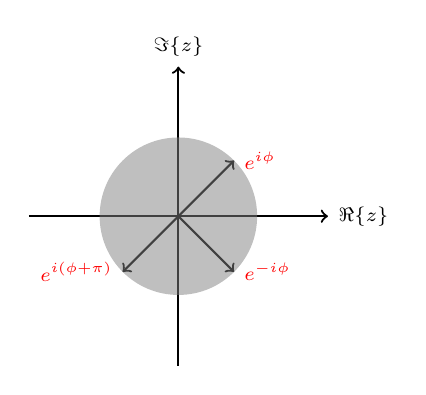
\begin{tikzpicture}
    \begin{scope}[thick,font=\scriptsize]
    %xscale=2
    % Axes:
    % Are simply drawn using line with the `->` option to make them arrows:
    % The main labels of the axes can be places using `node`s:
    \draw [->] (-1.9,0) -- (1.9,0) node [right]  {$\Re\{z\}$};
    \draw [->] (0,-1.9) -- (0,1.9) node [above] {$\Im\{z\}$};
    % Axes labels:
    % Are drawn using small lines and labeled with `node`s. The placement can be set using options

    % If you only want a single label per axis side:
    \draw [->] (0,0) -- (0.70710678118654746,0.70710678118654746) node [right]  {\textcolor{red}{$e^{i\phi}$}};
    \draw [->] (0,0) -- (-0.70710678118654746,-0.70710678118654746) node [left]  {\textcolor{red}{$e^{i(\phi+\pi)}$}};
    \draw [->] (0,0) -- (0.70710678118654746,-0.70710678118654746) node [right]  {\textcolor{red}{$e^{-i\phi}$}};

    \end{scope}
    % The circle is drawn with `(x,y) circle (radius)`
    % You can draw the outer border and fill the inner area differently.
    % Here I use gray, semitransparent filling to not cover the axes below the circle
    \path [draw=none,fill=gray,semitransparent] (0,0) circle (1);
\end{tikzpicture}
}
   \end{center}
   \caption{Unitary circle in the complex plane. In red, the corresponding angles of the polar representation $e^{i\phi}$.}
   \label{circle2}
 \end{wrapfigure}
From this equation we can quickly obtain some restrictions, namely
\begin{eqnarray}
    |a|e^{i(\theta+\phi)} + |b|e^{i(\chi+\phi')} = 1,\label{first}\\
    |a|e^{i(\theta-\phi)} +  |b|e^{i(\chi-\phi')} = 0.\label{second}
\end{eqnarray}
Taking eq. \ref{second} we can infer
\begin{equation*}
\begin{aligned}
    |a|e^{i(\theta-\phi)} &=-  |b|e^{i(\chi-\phi')} ,\\
    &= (-1)|b|e^{i(\chi-\phi')} ,\\
    &= (e^{-i\pi})|b|e^{i(\chi-\phi')} ,\\
    &= |b|e^{i(\chi-\phi'-\pi)}.
    \end{aligned}
\end{equation*}
This results in two conditions 
\begin{eqnarray}
    |a| = |b|, \label{cond1}\\
     \theta-\phi = \chi-\phi'-\pi. \label{cond2}
\end{eqnarray}
Using eq. \ref{cond1} in \ref{first} leads to
\begin{equation*}
\begin{aligned}
    1= |a|e^{i(\theta+\phi)} + |b|e^{i(\chi+\phi')} &= |a|e^{i(\theta+\phi)} + |a|e^{i(\chi+\phi')},\\
    & = |a|\left(e^{i(\theta+\phi)} + e^{i(\chi+\phi')}\right),
\end{aligned}
\end{equation*}
therefore
\begin{equation}
    \frac{1}{|a|} = e^{i(\theta+\phi)} + e^{i(\chi+\phi')}.\label{modExp}
\end{equation}
Last equation means that the right hand side must be purely real, since the left hand side is. As a consequence we can conclude that the imaginary part of $e^{i(\theta+\phi)}$ must be minus the imaginary part of $e^{i(\chi+\phi')}$ in order for them to cancel each other. This happens when either of the following two conditions is met 
\begin{equation}
    \theta+\phi = - (\chi+\phi'), \quad \text{ or } \quad\theta+\phi = \chi+\phi' + \pi \label{38}
\end{equation}
we can check this graphically in Fig. \ref{circle2}, or analitically using Euler's identity $e^{i\phi} = \cos(\phi) + i\sin(\phi)$
\begin{equation*}
\begin{aligned}
    e^{-i\phi} &= \cos(-\phi) + i\sin(-\phi),\\
     &= \cos(\phi) - i\sin(\phi).\\
     e^{i(\phi+\pi)} &= \cos(\phi+\pi) + i\sin(\phi+\pi),\\
     &= \cos(\phi)\cos(\pi) - \sin(\phi)\sin(\pi) + i(\sin(\phi)\cos(\pi) + \sin(\pi)\cos(\phi)),\\
     &= -\cos(\phi) - i\sin(\phi).
\end{aligned}
\end{equation*}
As we can see the second equation in \ref{38} would lead to zero in the right hand side of eq. \ref{modExp}. Hence we will discard that equation and use the other one. Our next step will be adding eqs. \ref{38} and \ref{cond2}
\begin{equation}
    \begin{aligned}[b]
        (\theta+\phi) + (\theta-\phi)&= - (\chi+\phi') + (\chi-\phi'-\pi),\\
        \Rightarrow 2\theta &= -2\phi' - \pi,\\
        \Rightarrow \theta &= -\phi' - \pi/2.
    \end{aligned}
    \label{42}
\end{equation}
If instead of adding them we subtract them the result will be 
\begin{equation}
    \begin{aligned}[b]
        (\theta+\phi) - (\theta-\phi)&= - (\chi+\phi') - (\chi-\phi'-\pi),\\
        \Rightarrow 2\phi &= -2\chi + \pi,\\
        \Rightarrow \chi &= -\phi - \pi/2.
    \end{aligned}
    \label{43}
\end{equation}
If we now go back to the first equation in \ref{38} and plug in eqs. \ref{42} and \ref{43} we will be able to find a relationship between the phase factors $\phi$ and $\phi'$
\begin{equation}
    \begin{aligned}[b]
        \theta+\phi &= - (\chi+\phi'),\\
        \Rightarrow -\phi' - \pi/2 +\phi &= -(-\phi - \pi/2)+\phi',\\
        -2\phi' +2\phi &= \pi,\\
        \phi - \phi' = \pi/2
    \end{aligned}
\end{equation}
In other words, if we want to recover the fermionic creation and annihilation operators $c_k$, $c_k^\dagger$ we have to choose a pair of Majorana operators $\gamma_k$, $\gamma_{k'}$ such that they have a phase difference of $\pi/2$. The simplest choice is $\phi=0$ and $\phi'=-\pi/2$, in this case the resulting operators are 
\begin{eqnarray}
    \gamma_k = e^{i0}c_k + e^{-i0}c_k^\dagger = c_k + c_k^\dagger,\nonumber \\
    \gamma_k = e^{-i\pi/2}c_k + e^{-i(-\pi/2)}c_k^\dagger = -ic_k +i c_k^\dagger = i(c_k^\dagger - c_k)\nonumber,
\end{eqnarray}
Just out of convention, and since both operators are associated with a single fermionic site, we label them as follows
\begin{eqnarray}
    \gamma_{2k-1} = c_k + c_k^\dagger,\label{def1}\\
    \gamma_{2k} = i(c_k^\dagger - c_k)\label{def2}.
\end{eqnarray}
From eqs. \ref{def1} and \ref{def2} we can now easily find how to express $c_k$ and $c_k^\dagger$
\begin{eqnarray}
    c_k = \frac{\gamma_{2k-1} + i \gamma_{2k}}{2},\label{cMaj}\\
    c_k^\dagger = \frac{\gamma_{2k-1} - i \gamma_{2k}}{2} \label{cMaj2}
\end{eqnarray}
We can then, finally, write the number operator
\begin{equation}
    \begin{aligned}[b]
        c_k^\dagger c_k &=  \left(\frac{\gamma_{2k-1} - i \gamma_{2k}}{2}\right) \left(\frac{\gamma_{2k-1} + i \gamma_{2k}}{2}\right),\\
        & = \frac{(\gamma_{2k-1} - i \gamma_{2k})(\gamma_{2k-1} + i \gamma_{2k})}{2},\\
        & = \frac{\gamma_{2k-1}\gamma_{2k-1} - i \gamma_{2k}\gamma_{2k-1} + i \gamma_{2k-1}\gamma_{2k} +  \gamma_{2k}\gamma_{2k}}{2},\\
        \text{using } \gamma_k^\dagger = \gamma_k \quad &= \frac{\gamma_{2k-1}^\dagger\gamma_{2k-1} - i \gamma_{2k}\gamma_{2k-1} + i \gamma_{2k-1}\gamma_{2k} +  \gamma_{2k}^\dagger\gamma_{2k}}{2},\\
        \text{using } \{\gamma_k,\gamma_l\} = 2\delta_{kl} \quad &= \frac{\gamma_{2k-1}^\dagger\gamma_{2k-1} - i \gamma_{2k}\gamma_{2k-1} - i \gamma_{2k}\gamma_{2k-1} +  \gamma_{2k}^\dagger\gamma_{2k}}{2},\\
        \text{using eq. \ref{quadOne}} \quad &= \frac{1 - 2i \gamma_{2k}\gamma_{2k-1} +  1}{2},\\
        &= \frac{2 - 2i \gamma_{2k}\gamma_{2k-1}}{2},\\
        &= 1 - i\gamma_{2k}\gamma_{2k-1}.
    \end{aligned}
    \label{numMaj}
\end{equation}

By now we should be a little familiar with the mathematics and the basic operators we need, but the physical meaning has been relegated. So it is a good time to highlight important concepts. In eqs. \ref{def1} and \ref{def2} its showed that a Majorana particle is born as a linear combination of creation and annihilation operators, this is, it consists of particles and holes in the same proportion. Also, as eqs. \ref{cMaj} and \ref{cMaj2} reveal, each fermion site has two Majorana particles associated to it. This might sound like a peculiarity, but we will see later that this are indeed fundamental properties.\\

Finally, we would like to discuss a little bit of what happens to our Majorana operators when we have gauge symmetry. In other words, what happens to $\gamma_{2k-1}$, and $\gamma_{2k}$ if $c_k$ and $c_k^\dagger$ satisfy
\begin{eqnarray}
    c_k \rightarrow e^{i\phi}c_k,\nonumber\\
    c_k^\dagger \rightarrow e^{-i\phi}c_k^\dagger.\nonumber
\end{eqnarray}
Let's check.
\begin{equation}
    \begin{aligned}[b]
        \gamma_{2k-1} = c_k + c_k^\dagger &\rightarrow e^{i\phi}c_k + e^{-i\phi}c_k^\dagger,\\
        &= (\cos(\phi) + i\sin(\phi))c_k + (\cos(-\phi) + i \sin(-\phi))c_k^\dagger,\\
        &= \cos(\phi)c_k + i\sin(\phi)c_k + \cos(\phi)c_k^\dagger - i \sin(\phi)c_k^\dagger,\\
        &= \cos(\phi)(c_k + c_k^\dagger) +\sin(\phi)(i(c_k -c_k^\dagger)),\\
        &= \cos(\phi)(c_k + c_k^\dagger) -\sin(\phi)(i(c_k^\dagger -c_k)),\\
        &= \cos(\phi)\gamma_{2k-1} -\sin(\phi)\gamma_{2k}.\label{mix1}
    \end{aligned}
\end{equation}
\begin{equation}
    \begin{aligned}[b]
        \gamma_{2k} = i(c_k^\dagger - c_k) &\rightarrow i(e^{-i\phi}c_k^\dagger - e^{i\phi}c_k),\\
        &= i((\cos(\phi) - i\sin(\phi))c_k^\dagger - (\cos(\phi) + i\sin(\phi))c_k),\\
        &= i\cos(\phi)c_k^\dagger  + \sin(\phi)c_k^\dagger - i\cos(\phi)c_k + \sin(\phi)c_k,\\
        &= \cos(\phi)(i(c_k^\dagger-c_k)) + \sin(\phi)(c_k + c_k^\dagger),\\\
        &= \cos(\phi)\gamma_{2k} + \sin(\phi)\gamma_{2k-1}.\label{mix2}
    \end{aligned}
\end{equation}
Physically this means that our modes are getting mixed, as a global phase is introduced. In contrast to the indifference fermions show against this symmetry, for Majorana modes there are physical consequences. Two special instances can be highlighted where this mixing can be avoided: by choosing $\phi=0$ or $\phi=\pi$.\footnote{This is a partial true, because $\pi/2$ and $3\pi/2$ wouldn't mix them, in these cases one operator is transformed into the other, one question then would be why do they ignore these cases usually when they want to break the symmetry?}\label{quest2} Naturally this is a property we would like to have, an interesting question we can pose to ourselves is then, is there a system bearing this symmetry? Well, long story short, yes.\\
